\documentclass{standalone}

\usepackage{tikz, pgf}

\begin{document}
    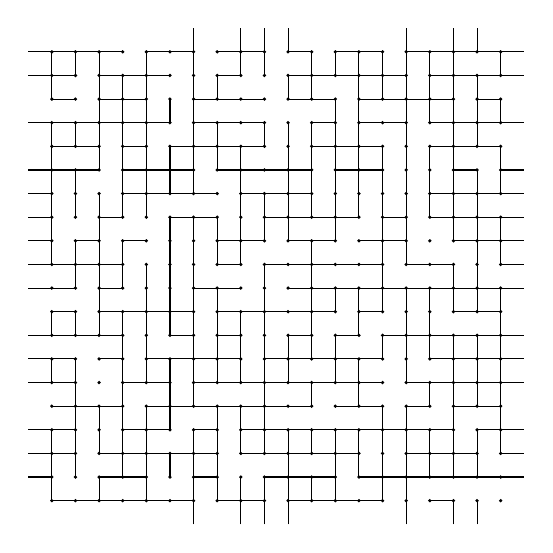
\begin{tikzpicture}[scale=0.30,every node/.style={draw,shape=circle,fill=black,inner sep=0pt,minimum size=0.75pt}]
      \pgfmathtruncatemacro\width{20}
      \pgfmathtruncatemacro\height{20}
      \foreach \i in {1,...,\width} {
        \foreach \j in {1,...,\height} {
          \path (\i,\j) node (a\i\j) {};
          \ifnum\j>1
            \pgfmathsetmacro\rand{rnd}
            \ifdim \rand pt<0.67pt
              \pgfmathsetmacro\k{\j -1}
              \draw (\i,\j) -- (\i,\k);
            \fi
          \fi
          \ifnum\j=1
            \pgfmathsetmacro\rand{rnd}
            \ifdim \rand pt<0.67pt
              \pgfmathsetmacro\k{\height +1}
              \draw(\i,0) -- (\i,1);
              \draw(\i,\height) -- (\i,\k);
            \fi
          \fi
          \ifnum\i>1
            \pgfmathsetmacro\rand{rnd}
            \ifdim \rand pt<0.67pt
              \pgfmathsetmacro\k{\i -1}
              \draw (\i,\j) -- (\k,\j);
            \fi
          \fi
          \ifnum\i=1
            \pgfmathsetmacro\rand{rnd}
            \ifdim \rand pt<0.67pt
              \pgfmathsetmacro\k{\width +1}
              \draw(0,\j) -- (1,\j);
              \draw(\height,\j) -- (\k,\j);
            \fi
          \fi
        }
      }
    \end{tikzpicture}
\end{document}

